\documentclass[14pt, a4paper] {ncc}
\usepackage[utf8] {inputenc}
\usepackage[T2A]{fontenc}
\usepackage[english, russian] {babel}
\usepackage[top=20mm, bottom=20mm, left=25mm, right=10mm]{geometry}
\usepackage{xcolor}
\usepackage{tikz}

\usepackage{biblatex}

% Для вставки фигур
\usepackage{float}
\usepackage{caption}

\usepackage{longtable,amsmath,amsfonts}

\usepackage{listings}
\usepackage{algpseudocode}
% More Math Symbols
\usepackage{stmaryrd}

% Enumeration
\usepackage{enumitem}
\setlist[enumerate]{topsep=0pt,itemsep=0ex,partopsep=1ex,parsep=1ex}
\setlist[itemize]{itemsep=0ex}

% Полуторный межстрочный интервал
\usepackage[nodisplayskipstretch]{setspace}
\onehalfspacing

% Добавить абзацный отступ для первых абзацев в section/subsection,
% по умолчанию не добавляется
\usepackage{indentfirst}

% Times New Roman
\usepackage{pscyr}
\renewcommand{\rmdefault}{ftm}


% Абзацный отступ равен 1.25 см
\parindent=1.25cm

% Номер страницы по середине верхнего поля
\usepackage{fancyhdr}
\pagestyle{fancy}
\fancyhf{}
\fancyhead[C]{\thepage}
\renewcommand{\headrulewidth}{0pt}


%%%%%%%%%%%%%%%%%%%%%%%%%
\lstdefinelanguage{MyLang}
{
  morekeywords={data},
  keywordstyle=\bfseries\color{black}
}
%%%%%%%%%%%%%%%%%%%%%%%%%
\newcommand{\larrow}{\leftarrow}
\newcommand{\rarrow}{\rightarrow}

\newcommand{\ukanren}{$\mu$Kanren }

\newcommand{\origin}[1]{(англ. {\it #1})}

\newcommand{\todo}[1]{{\bf\color{red}TODO: #1}}
%%%%%%%%%%%%%%%%%%%%%%%%%


\addbibresource{main.bib}

\begin{document}
\setcounter{figure}{0}

%\tableofcontents
%\newpage
%\section{Введение}

%\newpage
\section{Описание предметной области}

\subsection{Логическое и реляционное программирование}

{\bf Логическое программирование}~--- это вид декларативного программирования,
основанный на формальной логике. Программы представляются в виде
утверждений, представляющихся логическими формулами и описывающих
определённую область проблем.
``Вычисление'' программы в контексте логического программирования производится
в форме \emph{поиска} доказательства утверждений на основе заданных
фактов --- аксиом --- и правил вывода в соответствии с заданной
\emph{стратегией поиска}~\cite{logicMJ}.

Стратегия поиска задаёт,
каким образом происходит обход пространства поиска ответов, и,
как следствие, определяет как, какие и в каком порядке будут находиться
ответы. Стратегия поиска, при которой каждый возможный ответ будет со временем
выдан, называется \emph{полной}. Чаще применяются \emph{неполные} стратегии,
поскольку они менее требовательны к вычислительным ресурсам~\cite{currySearch}.

Самые известные языки логического программирования --- языки семейства Prolog.
Prolog применяется для доказательства теорем~\cite{prologTheorem},
проектирования баз знаний, создания экспертных систем~\cite{prologExSys}
и искусственного интеллекта~\cite{prologInt}.
Prolog строится на логике предикатов первого порядка в форме дизъюнктов
Хорна (то есть дизъюнктов только с одним положительным литералом) и
использует \emph{метод резолюций}, основанный на доказательстве от
противного, для решения задач.
Prolog вводит разнообразные синтаксические конструкции с
\emph{побочными эффектами}, то есть с действиями, приводящими к изменению
\emph{окружения} программы, к примеру, оперaтор отсечения~\origin{cut},
который влияет на способ вычисления программы, предотвращая нежелательные
вычисления.
Также он использует стратегию обхода в глубину, что приводит к тому, что
поиск может ``зациклиться'' и никогда не выдать оставшиеся решения,
но, тем не менее, благодаря своим расширениям Prolog
остаётся хорошим решением для задач из своей области применения~\cite{logicMJ}.

% Подобные операторы обычно используются для того, чтобы
% повысить эффективность программ, однако 

% Другие языки логического программровани, такие как Mercury\cite{mercury} или 
% Curry\cite{curry}, являются 

% {\bf Логическое программирование}~--- это вид декларативного программирования,
% основанный на логике предикатов первого порядка в форме дизъюнктов Хорна
% (то есть дизъюнктов
% с только одним положительным литералом),
% применяющий принципы логического вывода на основе заданных фактов и правил.
% Программа, написанная на логическом языке --- это множество логических формул,
% описывающих определённую область проблем.\cite{logicMJ}

% Существует множество языков логического программирования, таких как Prolog, Curry, Mercurry,
% однако самые известные --- языки семейства Prolog. Prolog применяется для доказательства
% теорем, проектирования баз знаний, создания экспертных систем и искусственного интеллекта.

% Prolog построен на \emph{методе резолюций}, который является обобщением метода
% ``доказательства от противного'', а в частности --- на \emph{линейном} методе
% резолюций \origin{Linear resolution with Selection function for Definition clauses}.
% При вычислении программы правило резолюции применяется не к случайных дизъюнктам,
% а в строго установленном порядке. В случае, когда вычисления дизъюнкта прошло
% неудачно, происходит \emph{откат} к прошлому состоянию программы, на котором
% выбирался неудавшийся дизъюнкт\cite{logicMJ}.
% 
% Помимо этого, Prolog вводит разнообразные синтаксические конструкции с побочными \emph{эффектами},
% то есть с действиями, приводящими к изменению \emph{окружения} программы,
% к примеру, оперaтор отсечения~\origin{cut},
% который влияет на способ вычисления программы.

% Это свойства определяют Prolog как язык, однако из-за них теряется свойство \emph{реляционности}.

% % 
% % Пример программы на Prolog приведён в Листинге~\ref{lst:memberProlog}.
% % 
% % \begin{lstlisting}[language=Prolog,caption={Проверка принадлежности элемента списку},captionpos=b,label={lst:memberProlog}]
% % member(X, [X | T]).
% % member(X, [H | T]) :- member(X, T).
% % \end{lstlisting}
% % 
% % В этой программе проверяется принадлежность элемента списку. Есть два возможных
% % варианта происходящего: либо элемент равен элементу в голове списка





{\bf Реляционное программирование}~--- это форма чистого логического
программирования, в котором программы задаются как набор
математических {\it отношений}. Реляционное программирование направлено
на получение \emph{значимых} ответов, как бы ни использовались отношения
~\cite{byrdMK}.

Исторически, понятие реляционного программирования появилось
раньше~\cite{relML} и задавало саму концепцию программы как отношения,
когда логическое --- появилось позже и предоставляло реализацию его
идей~\cite{logicMJ}.
Однако в данной работе под реляционным программированием понимается
непосредственно так, как указано выше.

В терминах реляционного программирования, к примеру, сложение $X + Y = Z$
может быть выражено отношением\footnote{Символ $\ ^o$ традиционно
используется для обозначения отношения.}
\[\text{add}^o (X, Y, Z),\]
которое в зависимости от того, какие переменные заданы, порождает
все возможные значения переменных, при которых отношение выполняется:
\begin{itemize}
\item \rel{add}(1, 2, 3) --- проверка выполнимости отношения;
\item \rel{add}(1, 2, A) --- поиск всех таких A, при которых 1 + 2 = A;
\item \rel{add}(A, B, 3) --- поиск всех таких A и B, при которых A + B = 3;
\item \rel{add}(A, B, C) --- поиск всех троек A, B и С, при которых A + B = C.
\end{itemize}

Чистые отношения не предполагают функциональных зависимостей между переменными,
поэтому поиск можно проводить в разных ``направлениях'', в зависимости от
того, какие переменные заданы, как показано выше в примере.

Когда же отношения вырождаются в функциональные и появляется
явная зависимость между переменными, тогда можно говорить про запуск
в ``прямом'' направлении --- то есть задаются входные аргументы --- и в
``обратном'' --- при задании результата.

К примеру, отношение ``меньше'' для двух чисел X и Y можно задавать как
\rel{less}(X, Y) и получить чистое реляционное отношение, либо
как \rel{$\text{less}_2$}(X, Y, R), где R сообщает, состоят ли X и Y
в отношении, и получить функциональное, и тогда задание X и Y будет
прямым направлением, а задание R --- обратным.

% Отличительная черта реляционного программирования в том, что с каким бы
% набором аргументов отношение ни было запущено, обязательно должны быть
% найдены все ответы, если они есть. Для сравнения, в Prolog 

% Ссылка на Булычева
Одно из применений реляционной парадигмы --- {\it реляционные интерпретаторы}.
Для языка $L$ его интерпретатор -- это функция $\text{eval}_L$, которая принимает
на вход программу $p_L$ на этом языке, её вход $i$ и возвращает некоторый выход $o$:
\[ \text{eval}_L (p_L, i) \equiv \llbracket p_L \rrbracket (i) = o \]
Реляционную версию интерпретатора можно представить как отношение:
\[ \text{eval}_L^o(p_L, i, o). \]

При запуске такого отношения в разных направлениях можно добиться интересных
эффектов: не только вычислять результат, но и по программе $p_L$ и выходу $o$
искать возможные входы $i$ или вовсе генерировать программу по указанным
выходам и входам.
% решать задачи поиска по задаче распознавания~\cite{lozov},
%генерировать программы по заданной спецификации входа $i$ и выхода $o$~\cite{unifiedMK}.

Можно отметить, что языках, основанных на классическом Prolog, производить
подобные вычисления для получения вразумительных результатов не получится. 


\subsection{miniKanren}

% Byrd
{\it miniKanren} -- семейство встраиваемых предметно-ориентированных языков,
специально спроектированное для реляционного программирования~\cite{byrdMK}.

Основная реализация miniKanren написана на языке Scheme~\cite{reasonedSchemer},
однако существует множество реализаций в ряде других языков, в том числе
Clojure, OCaml, Haskell и другие\footnote{\url{minikanren.org}}.

miniKanren предоставляет набор базовых конструкций: унификация ($\equiv$),
конъюнкция $(\land)$, дизъюнкция $(\lor)$, введение свежей переменной
(\lstinline{fresh}), вызов реляционного отношения,
--- представляющий ядро языка, и разнообразные расширения, к примеру, оператор неэквивалентности
\origin{disequality constraint} или нечистые операторы, предоставляющие функциональность
отсечения из Prolog. Несмотря на то, что в miniKanren введены операторы с эффектами, использование
его только с чистыми операторами предоставляет настоящую реляционность.

Классический пример --- программа конкатенации двух списков --- указан
на рисунке~\ref{fig:appendo}.

\begin{figure}[h!]
\begin{lstlisting}[mathescape,language=Haskell,extendedchars=\true,frame=single,basicstyle=\ttfamily]
$\text{append}^o$ X Y R =
  X $\equiv$ [] $\land$ Y $\equiv$ R $\lor$
  fresh (H X' R')
    (X $\equiv$ H :: X') $\land$
    (R $\equiv$ H :: R') $\land$
    $\text{appendo}^o$ X' Y R'
\end{lstlisting}

\caption{Пример программы на miniKanren (\lstinline{::} --- конструктор списка)}
\label{fig:appendo}
\end{figure}

Пояснение к программе:
список \lstinline{R} является конкатенацией списков \lstinline{X} и
\lstinline{Y} в случае, когда список \lstinline{X} пуст, а \lstinline{Y}
равен \lstinline{R}, либо когда \lstinline{X} и \lstinline{R} раскладываются
на голову и хвост, а их хвосты состоят в отношении конкатенации с \lstinline{Y}.

Для выполнения конкатенации над списками необходимо сформировать
\emph{запрос}~(или \emph{цель}).
В запросе в аргументах указываются либо замкнутые термы, либо термы
со свободными переменными. Результатом выполнения является список
подстановок для свободных переменных, при которых отношение выполняется;
когда свободных переменных нет, подстановка, соответственно, пустая.

На рисунке~\ref{fig:appendoExample} приведёт пример запроса, в котором мы хотим
найти возможные значения переменных \lstinline{Y} и \lstinline{R}. Потенциально
может быть бесконечное число ответов, к примеру, когда все аргументы в запросе
--- переменные, поэтому в системах miniKanren есть возможность запрашивать
несколько первых ответов; в примере, это число 1. Ответы могут содержать в себе
как конкретные замкнутые термы (к примеру, числа), так и свободные переменные,
которые в примере обозначаются как $\text{\_.}_n$. В примере одна и также
свободная переменная $\text{\_.}_0$ назначена и \lstinline{Y} и \lstinline{R}.
Это означает, что какое бы ни было значение \lstinline{Y}, оно всегда будет
являться хвостом \lstinline{R}.

\begin{figure}[h!]
\begin{lstlisting}[mathescape,language=Haskell,extendedchars=\true,frame=single,basicstyle=\ttfamily]
> run 1 (Y R) ($\text{append}^o$ [1, 2] Y R)
Y = $\text{\_.}_0$
R = 1 :: 2 :: $\text{\_.}_0$
\end{lstlisting}
\caption{Пример запуска отношения конкатенации.}
\label{fig:appendoExample}
\end{figure}

В определение miniKanren входит особый алгоритм поиска ответов --- чередующийся
поиск \origin{interleaving search}, основанный на поиске в глубину,
который рассматривает всё пространство поиска и является
полным~\cite{interleaving}.
% гарантирует, что если существует ответ, то алгоритм его предоставит за конечное время\cite{interleaving}.
%Для сравнения, обычный поиск в глубину, используемый в классическом Prolog при методе резолюций, может зациклиться
%или разойтись перед тем, как предоставить все ответы.
Это свойство чередующегося поиска определяет, вместе с отсутствием
нечистых расширений, реляционность miniKanren. 

% Применимость
Хотя miniKanren уже применяется в индустрии для поиска лечения редких
генетических заболеваний в точной медицине~\cite{medMK},
на данном этапе своего развития используется в основном в исследовательских
целях:
\begin{itemize}
\item реляционные интерпретаторы на miniKanren для решения задач поиска~\cite{lozov},
      техника программирования по примерам~\cite{unifiedMK};
\item для доказательство теорем~\cite{mkProver} ;
\item в области вычислительной лингвистики~\cite{mkLing}.
\end{itemize}

%Одно из интересных применений miniKanren --- {\it реляционные интерпретаторы}.
%Для языка $L$ его интерпретатор -- это функция $\text{eval}_L$, которая принимает
%на вход программу $p_L$ на этом языке, её вход $i$ и возвращает некоторый выход $o$:
%\[ \text{eval}_L (p_L, i) \equiv \llbracket p_L \rrbracket (i) = o,\]
%где $\llbracket \bullet \rrbracket $ --- семантика языка L.
%Тогда в miniKanren интерпретатор описывается отношением $\text{eval}^o_L(p_L, i, o)$.
%При запуске такого отношения на разном наборе аргументов можно добиться интересных эффектов:
%\begin{itemize}
%\item по программе $p_L$ и выходу $o$ искать возможные входы $i$ (запуск программы в обратном направлении);
%  %: $\text{eval}^o(\text{add}, I, 3)$
%\item решать задачи поиска по задаче распознавания~\cite{lozov};
%\item генерировать программы по заданной спецификации входа $i$ и выхода $o$
%(техника программирования по примерам)\cite{unifiedMK}.
%\end{itemize}

% \todo{проблемы miniKanren: долгое вычисления сложных алгоритмов, долгие вычисления в обратном направлении.}
Однако miniKanren обладает рядом существенных недостатков. Несмотря на то,
что он ближе всего подошёл к реализации чистой реляционности, вычислительно
он всё же зависим от сложности и ветвистости программ, из-за чего их запуск в
разных направлениях может работать с разной скоростью, в особенности запуск в обратном направлении,
который зачастую работает очень медленно.
Также, описывать сложные задачи в качестве отношений --- нетривиальная задача,
наивно написанные реляционные программы вычисляются крайне неэффективно.
Из-за чего, к примеру, сущестувет транслятор из функционального языка в
miniKanren~\cite{trconv}, однако порождаемые им отношения --- функциональные,
а запуск их в обратном направлении, как указывалось выше, крайне
непроизводителен~\cite{lozov}.

Одно из возможных решения проблем производительности --- специализация.


\subsection{Специализация}

{\bf Специализация} --- это метод автоматической оптимизации программ,
при которой из программы удаляются избыточные вычисления,
возможно, на основе информации о вхоных аргументах программы~\cite{jones}.

% Специализацию программ также называют \emph{частичными} или
% \emph{смешанными вычислениями}\cite{jones}.

{\it Специализатор} $\text{spec}_L$ языка $L$ принимает на вход программу $p_L$ и часть известного входа этой
программы $i_s$ (\emph{статических} данных) и генерирует новую программу $\hat{p}_L$, которая ведёт себя на оставшемся
входе $i_d$ (\emph{динамических} данных) также, как и оригинальная программа (формула~\ref{eq:spec}).

\begin{equation}
  \llbracket \text{spec}_L(p_L, i_s) \rrbracket (i_d) \equiv \hat{p}_L (i_d) \equiv \llbracket p_L \rrbracket (i_s, i_d)
\label{eq:spec}
\end{equation}

% Эффекты специализаторов
Специализатор производит все вычисления, зависимые от статических данных,
протягивание констант, инлайнгинг и другие.

Одно из интересных теоретических применений специализации --- это
\emph{проекции Футамуры}~\cite{futamura}. Процесс специализации интерпретатора
на программу на языке $L$ $\text{spec}_L(\text{eval}_L, p_L)$
порождает \emph{скомплированную} программу $\hat{p}_L$, а процесс специализации
специализатора на интерпретатор языка $L$
$\text{spec}_{L''}(\text{spec}_{L'}, \text{eval}_L)$, в свою очередь,
порождает \emph{компилятор}. Это первая и вторая проекции Футамуры
соответственно. Однако реализация специализаторов, которые бы не оставляли
в порождаемой программе следы интерпретации, сложная и труднодостижимая
задача~\cite{jones}.

Специализация разделяется на два больших класса: \emph{online} и \emph{offline}
алгоритмы:
\begin{itemize}
\item offline-cпециализаторы --- это двухфазовые алгоритмы специализации,
     в первой фазе которого происходит разметка исхного кода, к примеру,
     с помощью анализа времени связывания~\cite{jones}, и во второй
     фазе --- непосредственно во время специализации --- \emph{только}
     на основе полученной разметки принимаются решения об оптимизации;
\item online-специализаторы, напротив, принимают решения о специализации
      на лету и могут произвести вычисления, для которых offline сгенеировал
      бы код.
\end{itemize}

\todo{Связывающие слова.}

\subsubsection{Специализация логических языков}

{\bf Частичная дедукция} --- класс методов специализации логический языков,
основанных на построении деревьев вывода, которые отражают процесс вывода методом
резолюций, и анализе отдельно взятых атомов логических формул~\cite{advanced}.

Реализации методов частичной дедукции успешно применяются для
Prolog~\cite{prologPE},
в частности, система offline частичной дедукции LOGEN
показывает хорошие результаты при специализации интерпретаторов и
для некоторых интерпретаторов достигает для генерируемых программ
отсутствие накладных расходов на интерпретацию,
однако требует ручной модификации разметки~\cite{offlinePD}.

\Cpd --- одно из расширений метода частичной дедукции, отличительная
особенность которой состоит в том, что конъюнкции рассматриваются как
единая сущность наравне с атомами~\cite{cpd}. С помощью \forcpd
возможно добиться различных оптимизационных эффектов, среди которых
выделяется дефорестация~\origin{deforestation}~\cite{deforest}
--- оптимизация, при которой удаляются промежуточные структуры данных, ---
и таплинг~\origin{tupling}~\cite{tupling}
--- оптмизация, при которой множество проходов по одной структуре данных заменяется на один проход.
Это наиболее проработанный и мощный метод частичной дедукции.


Реализация методов частичной дедукции, включая конъюнктивную частичную дедукцию, для Prolog
представлена в виде системы ECCE~\cite{ecce}.

В работе~\cite{lozov} представляется адаптация конъюнктивной частичной дедукции для miniKanren.
Реализация добивается существенного роста производительности, однако,
как будет показано в разделе~\ref{src:testing}, в силу особенностей метода и его
направленности на Prolog, нестабильно даёт хорошие результаты и
в некоторых случаях может затормозить исполнение программы.

\subsubsection{Методы суперкомпиляции}
{\bf Суперкомпиляция} --- метод анализа и преобразования программ,
который отслеживает обобщённую возможную историю вычислений исходной программы и строит
на её основе эквивалентную ему программу, структура которой, в некотором смысле, ``проще''
структуры исходной программы. Впервые метод был предложен в работе \cite{turchinSC}.

Это упрощение достигается путём удаления или преобразования
некоторых избыточных действий: удаление лишнего кода, выполнение операций над
уже известными данными, избавление от промежуточных структур данных, инлайнинг,
превращение многопроходного алгоритма в однопроходный и другие. В конечном счёте,
суперкомпилятор может придать программе линейное ускорение\cite{scompRevisited}.

Суперкомпиляция включает в себя частичные вычисления, однако не сводится к ним полностью
и может привести в глубоким структурным изменениям оригинальной программы.

Суперкомпиляторы, которые используют только ``положительную'' информацию
--- то есть информацию о том, что сводобные переменные чему-то равны, ---
называют позитивными~\origin{positive supercompilation}\cite{scPos}.
К примеру, при достижении условного выражения {\bf if} x $=$ a {\bf then} $t_1$ {\bf else} $t_2$
позитивный суперкомпилятор при вычислении $t_1$ будет учитывать то, что x $=$ a,
однако при вычислении $t_2$ он не будет знать, что x $\neq$ a.
Расширение позитивного компилятора c поддержкой такой ``негативной'' информации --- идеальный
суперкомпилятор~\origin{perfect supercompilation}\cite{scPerf}.

Общая схема суперкомпилятора представлена на рисунке~\ref{fig:scompScheme}

\begin{figure}
\center
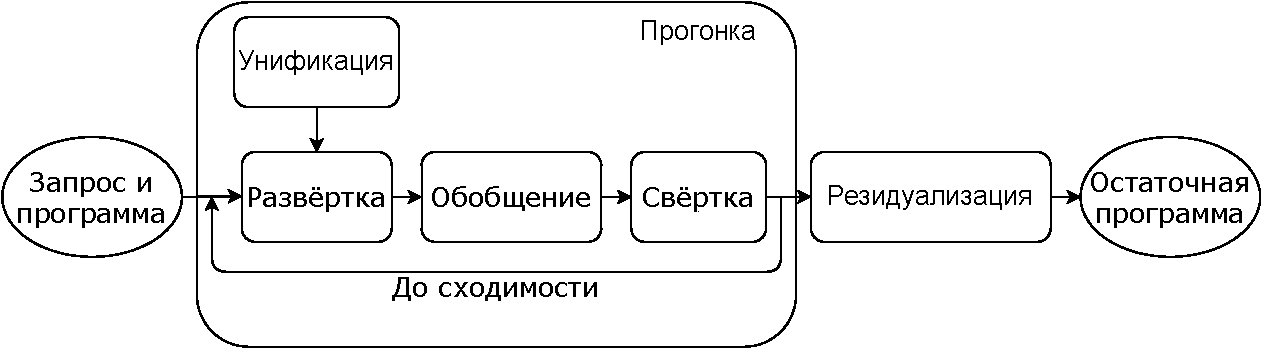
\includegraphics[scale=0.8]{./review/scompflow.pdf}
\caption{Общая схема суперкомпилятора.}
\label{fig:scompScheme}
\end{figure}

% Про "символьное исполнение" https://en.wikipedia.org/wiki/Symbolic_execution
% Сделать ссылку на Ключникова?
%История вычислений представляется в виде {\it графа конфигураций}, где {\it конфигурация}
%описывает состояние вычисления на конкретном шаге. Построение графа происходит на этапе
%{\it прогонки}, во время которого происходит символьное исполнение программы. Потенциально
%такой граф --- который без дополнительных шагов прогонки вырождается в дерево ---
%бесконечный. Для трансформации бесконечного дерева в конечный объект используется {\it cвёртка}
%--- при обработке конфигурации, выражение в которой является {\it переименованием} выражения в одной
%из родительских конфигураций.

История вычислений при суперкомпиляции представляется в виде \emph{графа процессов} --- корневого ориентированного графа,
в котором каждая ветвь --- это отдельный путь вычислений, а каждый узел --- состояние системы или \emph{конфигурация}.
Конфигурация обобщённо описывает множество состояний вычислительной системы или её подсистемы.
% К примеру, конфигурацией можно назвать пару из выражения $1 + x$, которое описывает все возможные суммы с $1$
% свободной переменной $x$, и множество органичений $\{ x \neq 10, x = 1 + x_1 \}$,
% которое сужает множество описываемых состояний до необходимого.
К примеру, конфигурацией можно назвать выражение $1 + x$, в котором параметр $x$ пробегает
все возможные значения своего домена (допустим, множество натуральных чисел) и задаёт
таким образом множество состояний программы\cite{turchinSC}.

Процесс построение графа процессов называется \emph{прогонкой}~\origin{driving}.
Во время прогонки производится шаг символьных вычислений, после которого
в граф процессов добавляются порождённые конфигурации; множество конфигураций
появляется тогда, когда ветвления в программе зависят от свободных переменных.

В процессе прогонки в конфигурациях могут появляться новые свободные переменные,
которые строятся из исходной конфигурации:
если при вычислении выражения его переменная перешла в другую переменную (к примеру, из-за сопоставления с образцом),
то в итоговую конфигурацию будет подставлена новая переменная и связь старой и новой сохранится в
некоторой \emph{подстановке}.
Подстановка --- это отображение из множества переменных в множество возможно замкнутых термов.
Применение подстановки к выражению заменит все вхождения переменных, принадлежащих её домену,
на соответствующие термы. %\todo{Что-нибудь ещё}

Пример графа процессов представлен на рисунке~\ref{fig:pgraphExample}.
\begin{figure}[h!]
\center
\begin{tikzpicture}[->,node distance=3cm, sibling distance=5cm]
                                                            
  \tikzstyle{conf}=[rectangle,draw, rounded corners=.8ex]

  \node[conf] (root) {$(a + b) + c$} ;
  \node[conf] (childLeft) [below left of = root] {$b + c$};
  \node[conf] (childRight)[below right of = root] {$(\text{Succ}(a_1) + b) + c$};
  \path (root) edge node[above left,pos=1] {$\{a \mapsto \text{Zero}\}$} (childLeft)
        (root) edge node[above right,pos=1]{$\{a \mapsto \text{Succ}(a_1)\}$}(childRight);
\end{tikzpicture}

\caption{Пример части графа процессов.}
\label{fig:pgraphExample}
\end{figure}
Здесь при исполнении выражение $(a + b) + c$, где $a, b, c$ -- натуральные числа,
были рассмотрены возможные значения $a$: это либо оно равно нулю (конструктор Zero), либо это некоторое
число $a_1$, которому прибавили единицу (конструктор Succ). Эти два случая могут задают
различные пути исполнения и, соответственно, добавлены в дерево процессов как два различных состояния,
в одно из которых войдёт программа при исполнении.



Потенциально процесс прогонки бесконечный, к примеру, когда происходят рекурсивные вызовы.
Для превращения бесконечого дерева вычисления в конечный объект, по которому множно
восстановить исходное дерево, используется \emph{свёртка.}

Свёртка~\origin{folding}~--- это процесс преобразования дерева процессов в граф, при котором
из вершины $v_c$ добавляется ребро в родительскую вершину $v_p$,
если выражение в конфигурации в $v_c$ и в $v_p$ равны с точностью до переименования.
Пример ситуации для свёртки изображён на рисунке~\ref{fig:pgraphFoldingExample},
на котором свёрточное ребро изображено пунктиром.

\begin{figure}[h!]
\center
\begin{tikzpicture}[->,node distance=2.3cm, sibling distance=5cm]
                                                            
  \tikzstyle{conf}=[rectangle,draw, rounded corners=.8ex]

  \node[conf] (root) {$a + b$} ;
  \node[conf] (childLeft) [below left of = root] {$b$};
  \node[conf] (childRight)[below right of = root] {$(\text{Succ}(a_1) + b)$};
  \node[conf] (childRight2)[below  of = childRight] {$(a_1 + b)$};
  \node (left)[below of = childLeft] {$\cdots$};

  \path (root) edge node[above left,pos=1] {$\{a \mapsto \text{Zero}\}$} (childLeft)
        (root) edge node[above right,pos=1]{$\{a \mapsto \text{Succ}(a_1)\}$}(childRight)
        (childLeft) edge (left)
        (childRight) edge (childRight2)
        (childRight2) edge[bend right=90] (root);
\end{tikzpicture}

\caption{Пример свёртки.}
\label{fig:pgraphFoldingExample}
\end{figure}

Однако существует ситуации, при котором свёртка не приведёт к тому, что граф превратится в
конечный объект. Такое может произойти, к примеру, когда два выражения структурно
схожи, но не существует переименования, уравнивающих их: $a + b$ и $a + a$.

Для решения этой проблемы используется \emph{обобщение}\cite{scGen}. Обобщение --- это процесс
замены одной конфигурации на другую, более абстрактную, описывающую больше состояний
программы. Для обнаружения ``похожей'' конфигурации используется предикат,
традиционно называемый \emph{свистком}: свисток пробегает по всем
родителям текущей конфигурации и определяет, похожа ли конфигурация на кого-то из них.
В случае, когда свисток сигнализирует о найденной схожести, применяется обобщение.
Сам шаг обобщения может произвести действия трёх видов:
\begin{itemize}
\item \emph{обобщение вниз} приводит к тому, что новая конфигурация заменяет текущую в графе процессов;
\item \emph{обобщение вверх} приводит к замене родительской конфигурации на обобщённую;
\item \emph{разделение}~\origin{split} используется для декомпозиции выражении, элементы которого затем
будут обработаны отдельно.
\end{itemize}
Пример обобщения представлен на рисунке~\ref{fig:pgraphGenExample}

\begin{figure}[h!]
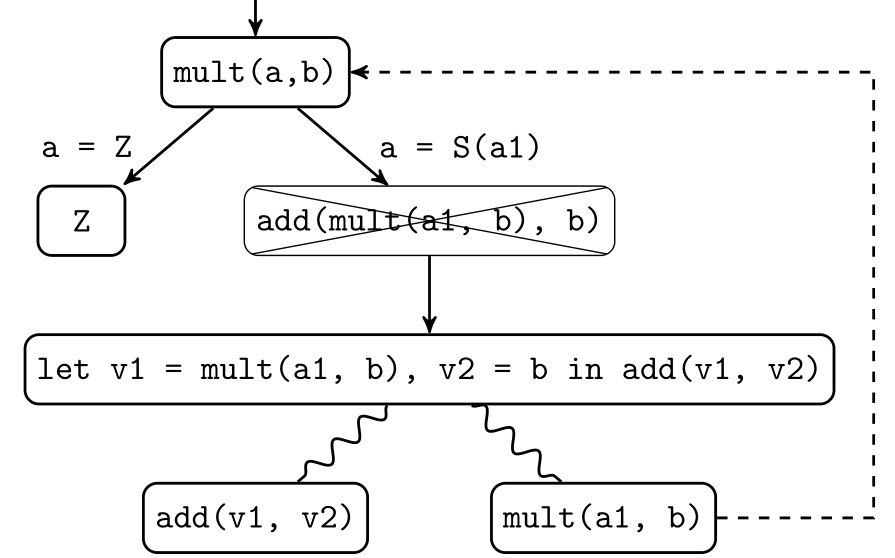
\includegraphics[scale=0.3]{./review/scgenex_temp.png}
\caption{Пример обобщения \todo{свой рисунок}.}
\label{fig:pgraphGenExample}
\end{figure}

Построение программы по графу конфигураций называется \emph{резидуализацией}, а
построенная программа --- \emph{остаточной} \origin{residual}.
Алгоритм выявления остаточной программы основан на обходе дерева, но
в остальном полностью зависит от языка.

% \todo{Написать ещё про СК; продемонстрировать результаты СК; выводы}

Техника суперкомпиляции применяется для функциональных\cite{scHaskell, scPos}
и императивных\cite{scJava} языков. \todo{Кажется, нужны какие-то выводы}



\subsection{Суперкомпиляция}

{\bf Суперкомпиляция} --- метод анализа и преобразования программ,
который отслеживает обобщённую возможную историю вычислений исходной программы и строит
на её основе эквивалентную ему программу, структура которой, в некотором смысле, ``проще''
структуры исходной программы. Впервые метод был предложен в работе \cite{turchinSC}.

Это упрощение достигается путём удаления или преобразования
некоторых избыточных действий: удаление лишнего кода, выполнение операций над
уже известными данными, избавление от промежуточных структур данных, инлайнинг,
превращение многопроходного алгоритма в однопроходный и другие. В конечном счёте,
суперкомпилятор может придать программе линейное ускорение\cite{scompRevisited}.

Суперкомпиляция включает в себя частичные вычисления, однако не сводится к ним полностью
и может привести в глубоким структурным изменениям оригинальной программы.

Суперкомпиляторы, которые используют только ``положительную'' информацию
--- то есть информацию о том, что сводобные переменные чему-то равны, ---
называют позитивными~\origin{positive supercompilation}\cite{scPos}.
К примеру, при достижении условного выражения {\bf if} x $=$ a {\bf then} $t_1$ {\bf else} $t_2$
позитивный суперкомпилятор при вычислении $t_1$ будет учитывать то, что x $=$ a,
однако при вычислении $t_2$ он не будет знать, что x $\neq$ a.
Расширение позитивного компилятора c поддержкой такой ``негативной'' информации --- идеальный
суперкомпилятор~\origin{perfect supercompilation}\cite{scPerf}.

Общая схема суперкомпилятора представлена на рисунке~\ref{fig:scompScheme}

\begin{figure}
\center
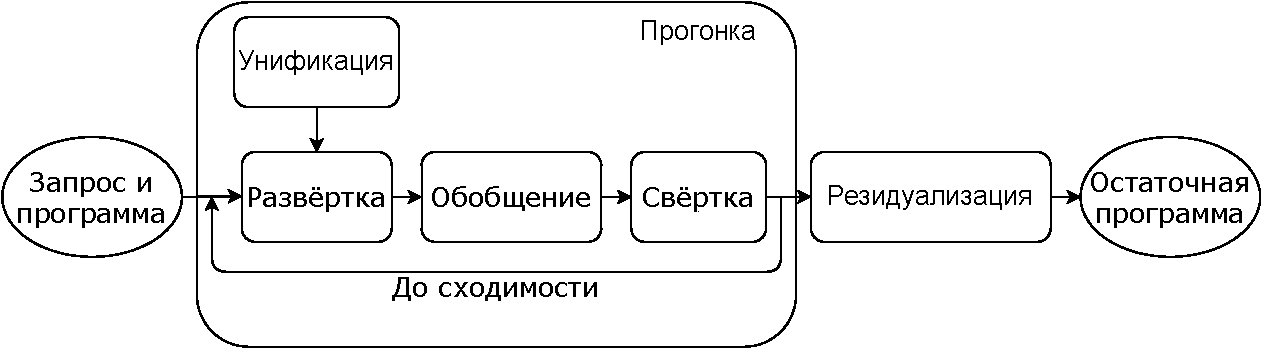
\includegraphics[scale=0.8]{./review/scompflow.pdf}
\caption{Общая схема суперкомпилятора.}
\label{fig:scompScheme}
\end{figure}

% Про "символьное исполнение" https://en.wikipedia.org/wiki/Symbolic_execution
% Сделать ссылку на Ключникова?
%История вычислений представляется в виде {\it графа конфигураций}, где {\it конфигурация}
%описывает состояние вычисления на конкретном шаге. Построение графа происходит на этапе
%{\it прогонки}, во время которого происходит символьное исполнение программы. Потенциально
%такой граф --- который без дополнительных шагов прогонки вырождается в дерево ---
%бесконечный. Для трансформации бесконечного дерева в конечный объект используется {\it cвёртка}
%--- при обработке конфигурации, выражение в которой является {\it переименованием} выражения в одной
%из родительских конфигураций.

История вычислений при суперкомпиляции представляется в виде \emph{графа процессов} --- корневого ориентированного графа,
в котором каждая ветвь --- это отдельный путь вычислений, а каждый узел --- состояние системы или \emph{конфигурация}.
Конфигурация обобщённо описывает множество состояний вычислительной системы или её подсистемы.
% К примеру, конфигурацией можно назвать пару из выражения $1 + x$, которое описывает все возможные суммы с $1$
% свободной переменной $x$, и множество органичений $\{ x \neq 10, x = 1 + x_1 \}$,
% которое сужает множество описываемых состояний до необходимого.
К примеру, конфигурацией можно назвать выражение $1 + x$, в котором параметр $x$ пробегает
все возможные значения своего домена (допустим, множество натуральных чисел) и задаёт
таким образом множество состояний программы\cite{turchinSC}.

Процесс построение графа процессов называется \emph{прогонкой}~\origin{driving}.
Во время прогонки производится шаг символьных вычислений, после которого
в граф процессов добавляются порождённые конфигурации; множество конфигураций
появляется тогда, когда ветвления в программе зависят от свободных переменных.

В процессе прогонки в конфигурациях могут появляться новые свободные переменные,
которые строятся из исходной конфигурации:
если при вычислении выражения его переменная перешла в другую переменную (к примеру, из-за сопоставления с образцом),
то в итоговую конфигурацию будет подставлена новая переменная и связь старой и новой сохранится в
некоторой \emph{подстановке}.
Подстановка --- это отображение из множества переменных в множество возможно замкнутых термов.
Применение подстановки к выражению заменит все вхождения переменных, принадлежащих её домену,
на соответствующие термы. %\todo{Что-нибудь ещё}

Пример графа процессов представлен на рисунке~\ref{fig:pgraphExample}.
\begin{figure}[h!]
\center
\begin{tikzpicture}[->,node distance=3cm, sibling distance=5cm]
                                                            
  \tikzstyle{conf}=[rectangle,draw, rounded corners=.8ex]

  \node[conf] (root) {$(a + b) + c$} ;
  \node[conf] (childLeft) [below left of = root] {$b + c$};
  \node[conf] (childRight)[below right of = root] {$(\text{Succ}(a_1) + b) + c$};
  \path (root) edge node[above left,pos=1] {$\{a \mapsto \text{Zero}\}$} (childLeft)
        (root) edge node[above right,pos=1]{$\{a \mapsto \text{Succ}(a_1)\}$}(childRight);
\end{tikzpicture}

\caption{Пример части графа процессов.}
\label{fig:pgraphExample}
\end{figure}
Здесь при исполнении выражение $(a + b) + c$, где $a, b, c$ -- натуральные числа,
были рассмотрены возможные значения $a$: это либо оно равно нулю (конструктор Zero), либо это некоторое
число $a_1$, которому прибавили единицу (конструктор Succ). Эти два случая могут задают
различные пути исполнения и, соответственно, добавлены в дерево процессов как два различных состояния,
в одно из которых войдёт программа при исполнении.



Потенциально процесс прогонки бесконечный, к примеру, когда происходят рекурсивные вызовы.
Для превращения бесконечого дерева вычисления в конечный объект, по которому множно
восстановить исходное дерево, используется \emph{свёртка.}

Свёртка~\origin{folding}~--- это процесс преобразования дерева процессов в граф, при котором
из вершины $v_c$ добавляется ребро в родительскую вершину $v_p$,
если выражение в конфигурации в $v_c$ и в $v_p$ равны с точностью до переименования.
Пример ситуации для свёртки изображён на рисунке~\ref{fig:pgraphFoldingExample},
на котором свёрточное ребро изображено пунктиром.

\begin{figure}[h!]
\center
\begin{tikzpicture}[->,node distance=2.3cm, sibling distance=5cm]
                                                            
  \tikzstyle{conf}=[rectangle,draw, rounded corners=.8ex]

  \node[conf] (root) {$a + b$} ;
  \node[conf] (childLeft) [below left of = root] {$b$};
  \node[conf] (childRight)[below right of = root] {$(\text{Succ}(a_1) + b)$};
  \node[conf] (childRight2)[below  of = childRight] {$(a_1 + b)$};
  \node (left)[below of = childLeft] {$\cdots$};

  \path (root) edge node[above left,pos=1] {$\{a \mapsto \text{Zero}\}$} (childLeft)
        (root) edge node[above right,pos=1]{$\{a \mapsto \text{Succ}(a_1)\}$}(childRight)
        (childLeft) edge (left)
        (childRight) edge (childRight2)
        (childRight2) edge[bend right=90] (root);
\end{tikzpicture}

\caption{Пример свёртки.}
\label{fig:pgraphFoldingExample}
\end{figure}

Однако существует ситуации, при котором свёртка не приведёт к тому, что граф превратится в
конечный объект. Такое может произойти, к примеру, когда два выражения структурно
схожи, но не существует переименования, уравнивающих их: $a + b$ и $a + a$.

Для решения этой проблемы используется \emph{обобщение}\cite{scGen}. Обобщение --- это процесс
замены одной конфигурации на другую, более абстрактную, описывающую больше состояний
программы. Для обнаружения ``похожей'' конфигурации используется предикат,
традиционно называемый \emph{свистком}: свисток пробегает по всем
родителям текущей конфигурации и определяет, похожа ли конфигурация на кого-то из них.
В случае, когда свисток сигнализирует о найденной схожести, применяется обобщение.
Сам шаг обобщения может произвести действия трёх видов:
\begin{itemize}
\item \emph{обобщение вниз} приводит к тому, что новая конфигурация заменяет текущую в графе процессов;
\item \emph{обобщение вверх} приводит к замене родительской конфигурации на обобщённую;
\item \emph{разделение}~\origin{split} используется для декомпозиции выражении, элементы которого затем
будут обработаны отдельно.
\end{itemize}
Пример обобщения представлен на рисунке~\ref{fig:pgraphGenExample}

\begin{figure}[h!]
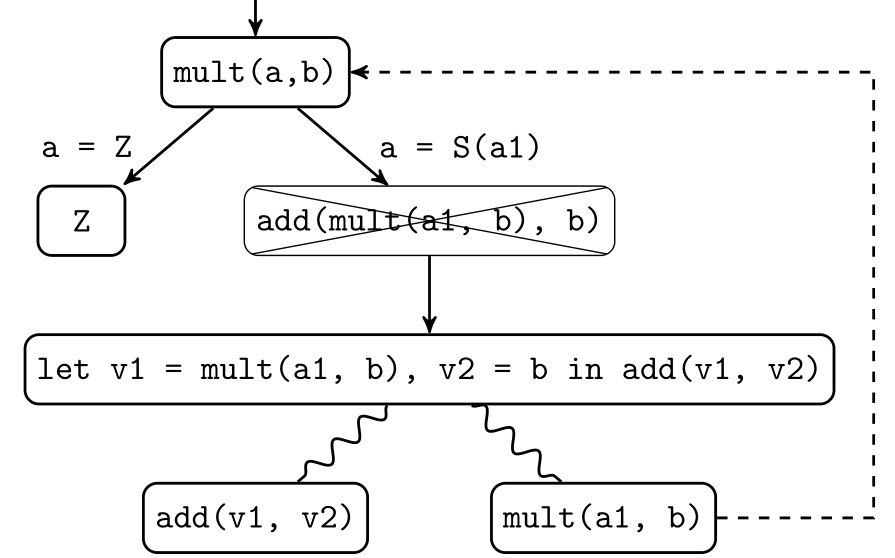
\includegraphics[scale=0.3]{./review/scgenex_temp.png}
\caption{Пример обобщения \todo{свой рисунок}.}
\label{fig:pgraphGenExample}
\end{figure}

Построение программы по графу конфигураций называется \emph{резидуализацией}, а
построенная программа --- \emph{остаточной} \origin{residual}.
Алгоритм выявления остаточной программы основан на обходе дерева, но
в остальном полностью зависит от языка.

% \todo{Написать ещё про СК; продемонстрировать результаты СК; выводы}

Техника суперкомпиляции применяется для функциональных\cite{scHaskell, scPos}
и императивных\cite{scJava} языков. \todo{Кажется, нужны какие-то выводы}


%\newpage
\section{Специализация miniKanren}

В данной работе для специализации был выбран \ukanren --- минималистичный диалект языка miniKanren\cite{uKanren}.
\ukanren содержит только чистые операторы, что заначительно упрощает процесс специализации.

Абстрактный cинтаксис языка представлен на Рисунке~\ref{fig:syntax}.

\begin{figure}[h!]
\centering
\[\begin{array}{ccll}
  \mathcal{C}   & = & \{C_i\}                                                   &\mbox{конструктор с арностью}\ i \\
  \mathcal{X}   & = & \{ x, y, z, \dots \}                                      &\mbox{переменные} \\
  \mathcal{T}_X & = & X \cup \{C_i (t_1, \dots, t_i) \mid t_j\in\mathcal{T}_X\} &\mbox{термы над множеством переменных $X$} \\
  \mathcal{D}   & = & \mathcal{T}_\emptyset                                     &\mbox{замкнутое выражение}\\
  \mathcal{R}   & = & \{ R_i\}                                                  &\mbox{реляционный символ с арностью}\ i \\[2mm]
  \mathcal{G}   & = & \mathcal{T_X}\equiv\mathcal{T_X}                          &\mbox{унификация} \\
                &   & \mathcal{G}\land\mathcal{G}                               &\mbox{конъюнкция} \\
                &   & \mathcal{G}\lor\mathcal{G}                                &\mbox{дизъюнкция} \\
                &   & \mbox{\lstinline|fresh|}\;\mathcal{X}\;.\;\mathcal{G}     &\mbox{введение свежей переменной} \\
                &   & R_i (t_1,\dots,t_i),\;t_j\in\mathcal{T_X}                 &\mbox{вызов реляционного отношения} \\[2mm]
  \mathcal{S}   & = & \{R_i^j = \lambda\;x_1\dots x_i\,.\, g_j;\}\; g           &\mbox{спецификация программы}
\end{array}\]
\caption{Синтаксис языка \ukanren\cite{semanticMK}.}
\label{fig:syntax}
\end{figure}

\begin{itemize}
\item Унификация двух термов $t_1 \equiv t_2$ порождает подстановку $\theta$, называемую \emph{унификатором},
      такую что её применение к термам уравнивает их: $t_1 \theta = t_2 \theta$.

      Алгоритм унификации языков семейства miniKanren использует проверку вхождения \origin{occurs check},
      что гарантирует корректность получаемых унификаторов, однако довольно сильно замедляет выполнение программ.

\item Конъюнкция двух целей $g_1 \land g_2$ подразумевает одновременное успешное выполнение выражений $g_1$ и $g_2$.
\item Дизъюнкция двух целей $g_1 \lor g_2$ подразумевает, что достаточно, чтобы хотя бы одно из выражений $g_1$ или $g_2$ выполнялось успешно.
      Следует отметить, что при выполнении $g_1$ выражение $g_2$ также будет вычисляться.
\item Введение свежей переменной $\text{fresh}\ x\ .\ g$ в языках miniKanren нужно указывать явно, в отличие, к примеру,
      от Prolog, где это происходит неявно.
\item Вызов реляционного отношения приводит к тому, что переданные в отношение термы
      унифицируются со аргументами отношения и подставляются в тело отношения. 
\end{itemize}

В контексте вычислений важно различие между \emph{синтаксическими} переменными, которые
определяются в тексте программы и обычно представляются строковыми литералами, и
\emph{семантическими} переменными, которые непосредственно используются в процессе вычислений и
представляются целыми числами, с которыми легче работать и генерировать свежие.

\ukanren является ядром языка miniKanren и может быть без труда расширен необходимыми
конструкциями.


\subsection{Реализация суперкомпиляции}
Реализация суперкомпилятора для \ukanren строилась на основе проекта
по специализации miniKanren на основе конъюнктивной частичной
дедукции\footnote{\url{https://github.com/kajigor/uKanren_transformations/}}.


%\section{Алгоритм суперкомпиляции}
% \begin{figure}[h!]
% \begin{lstlisting}[mathescape,language=MyLang]
%   data Tree where
%     Failure     :: Tree
%     Success     :: Substitution $\rarrow$ Tree
%     Abstraction :: Expression $\rarrow$ Substitution $\rarrow$ Tree
%     Unfolding   :: Expression $\rarrow$ Substitution $\rarrow$ Tree
%     Renaming    :: Expression $\rarrow$ Substitution $\rarrow$ Tree
% \end{lstlisting}
% \end{figure}
% 
% 
% \begin{figure}[h!]
% \begin{algorithmic}
% \Function{drive}{tree, expression}
%   \If {expression is renaming of some parent in the tree}
%     \State {add leaf to tree}
%   \ElsIf {$\exists \text{parent}:$ parent is embeded in expression}
%     \State {add abstraction node in tree}
%     \State {abstracted-expr <- abstract expression (parents in tree)}
%     \ForAll{expr : abstracted-expr}
%       \State \Call{drive}{tree, expr}
%     \EndFor
%   \Else
%     \State {children <- unfold expression}
%     \State {add unfolding node in tree}
%     \ForAll{child : children}
%       \State \Call{drive}{tree, child}
%     \EndFor
%   \EndIf
% \EndFunction
% \end{algorithmic}
% \caption{Базовый алгоритм прогонки}
% \end{figure}
% 

%\newpage
\section{Реализация и тестирование}

\subsection{Тестирование}

В качестве конкретной реализации \ukanren для тестирования
использовался OCanren (ссылка).

Cуперкомпиляторы реализованы на основе реализации CPD для miniKanren.

%\newpage
%\section{Заключение}


\end{document}
